\documentclass[a4paper,3p,sort&compress]{elsarticle}%
\usepackage[T1]{fontenc}%
\usepackage[utf8]{inputenc}%
\usepackage{lmodern}%
\usepackage{textcomp}%
\usepackage{lastpage}%
\usepackage{subcaption}%
%
\usepackage{tikz}%
\usepackage{pgfplots}%
\usepgfplotslibrary{external}%
\tikzexternalize[prefix=tikz_figures/]%
\newcommand{\inputtikz}[1]{\tikzsetnextfilename{#1}\input{tikz_files/#1.tikz}}%
\pgfplotsset{every axis/.append style={label style={font=\tiny},tick label style={font=\tiny},axis lines*=left,axis line style={-},}}%
\pgfplotsset{every add plot/.append style={line width=1pt,}}%
\usepackage{xcolor}%
\definecolor{blue}{HTML}{95DBE5}%
\definecolor{red}{HTML}{078282}%
\definecolor{green}{HTML}{339E66}%
%
\begin{document}%
\normalsize%


\begin{figure}[h!]%
\centering%
\begin{subfigure}[b]{0.25\textwidth}%
\centering%
\inputtikz{geo/g1021_mesh}%
\caption{Ex. V: geometry}%
\end{subfigure}%
\begin{subfigure}[b]{0.25\textwidth}%
\centering%
\inputtikz{geo/g1121_mesh}%
\caption{Ex. VI: geometry}%
\end{subfigure}%
\begin{subfigure}[b]{0.25\textwidth}%
\centering%
\inputtikz{geo/g1501_mesh}%
\caption{Ex. VII: geometry}%
\end{subfigure}%
\begin{subfigure}[b]{0.25\textwidth}%
\centering%
\inputtikz{geo/g1311_mesh}%
\caption{Ex. VIII: geometry}%
\end{subfigure}%
\\%
\begin{subfigure}[b]{0.25\textwidth}%
\centering%
\resizebox{\textwidth}{!}{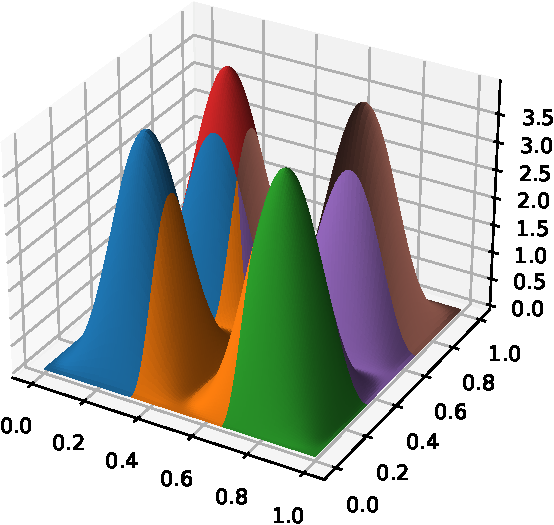
\includegraphics[width=\textwidth]{tikz_figures/geo/solution_g1021.pdf}%
}%
\caption{Ex. V: solution}%
\end{subfigure}%
\begin{subfigure}[b]{0.25\textwidth}%
\centering%
\resizebox{\textwidth}{!}{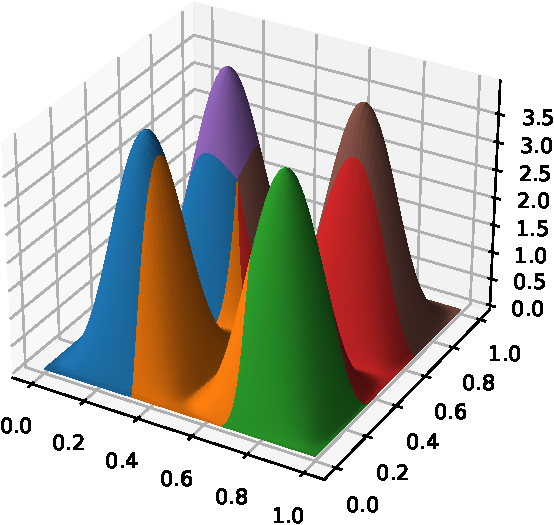
\includegraphics[width=\textwidth]{tikz_figures/geo/solution_g1121.pdf}%
}%
\caption{Ex. VI: solution}%
\end{subfigure}%
\begin{subfigure}[b]{0.25\textwidth}%
\centering%
\resizebox{\textwidth}{!}{\includegraphics[width=\textwidth]{tikz_figures/geo/solution_g1501.pdf}%
}%
\caption{Ex. VII: solution}%
\end{subfigure}%
\begin{subfigure}[b]{0.25\textwidth}%
\centering%
\resizebox{\textwidth}{!}{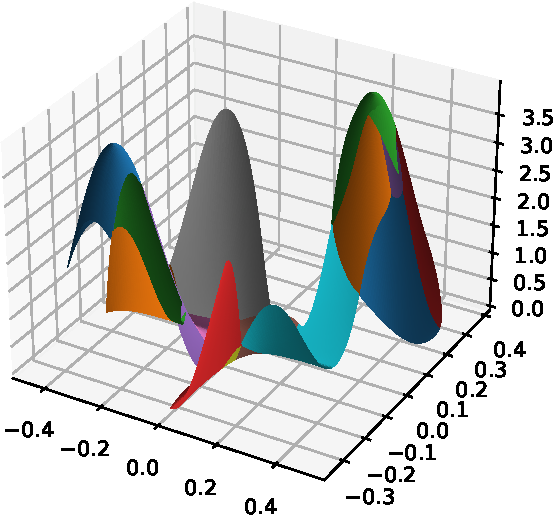
\includegraphics[width=\textwidth]{tikz_figures/geo/solution_g1311.pdf}%
}%
\caption{Ex. VIII: solution}%
\end{subfigure}%
\\%
\caption{Two kittens}%
\end{figure}

%
\end{document}